\documentclass[11pt,a4paper,]{article}
\usepackage{lmodern}

\usepackage{amssymb,amsmath}
\usepackage{ifxetex,ifluatex}
\usepackage{fixltx2e} % provides \textsubscript
\ifnum 0\ifxetex 1\fi\ifluatex 1\fi=0 % if pdftex
  \usepackage[T1]{fontenc}
  \usepackage[utf8]{inputenc}
\else % if luatex or xelatex
  \usepackage{unicode-math}
  \defaultfontfeatures{Ligatures=TeX,Scale=MatchLowercase}
\fi
% use upquote if available, for straight quotes in verbatim environments
\IfFileExists{upquote.sty}{\usepackage{upquote}}{}
% use microtype if available
\IfFileExists{microtype.sty}{%
\usepackage[]{microtype}
\UseMicrotypeSet[protrusion]{basicmath} % disable protrusion for tt fonts
}{}
\PassOptionsToPackage{hyphens}{url} % url is loaded by hyperref
\usepackage[unicode=true]{hyperref}
\hypersetup{
            pdftitle={Spatial modelling of the two-party preferred vote in Australian federal elections: 2001--2016},
            pdfkeywords={federal election, Census, Australia, spatial modelling, imputation, socio-demographics, electorates, R, eechidna},
            pdfborder={0 0 0},
            breaklinks=true}
\urlstyle{same}  % don't use monospace font for urls
\usepackage{geometry}
\geometry{left=2.5cm,right=2.5cm,top=2.5cm,bottom=2.5cm}
\usepackage[style=authoryear-comp,]{biblatex}
\addbibresource{references.bib}
\usepackage{longtable,booktabs}
% Fix footnotes in tables (requires footnote package)
\IfFileExists{footnote.sty}{\usepackage{footnote}\makesavenoteenv{long table}}{}
\IfFileExists{parskip.sty}{%
\usepackage{parskip}
}{% else
\setlength{\parindent}{0pt}
\setlength{\parskip}{6pt plus 2pt minus 1pt}
}
\setlength{\emergencystretch}{3em}  % prevent overfull lines
\providecommand{\tightlist}{%
  \setlength{\itemsep}{0pt}\setlength{\parskip}{0pt}}
\setcounter{secnumdepth}{5}

% set default figure placement to htbp
\makeatletter
\def\fps@figure{htbp}
\makeatother


\title{Spatial modelling of the two-party preferred vote in Australian federal elections: 2001--2016}

%% MONASH STUFF

%% CAPTIONS
\RequirePackage{caption}
\DeclareCaptionStyle{italic}[justification=centering]
 {labelfont={bf},textfont={it},labelsep=colon}
\captionsetup[figure]{style=italic,format=hang,singlelinecheck=true}
\captionsetup[table]{style=italic,format=hang,singlelinecheck=true}

%% FONT
\RequirePackage{bera}
\RequirePackage{mathpazo}

%% HEADERS AND FOOTERS
\RequirePackage{fancyhdr}
\pagestyle{fancy}
\rfoot{\Large\sffamily\raisebox{-0.1cm}{\textbf{\thepage}}}
\makeatletter
\lhead{\textsf{\expandafter{\@title}}}
\makeatother
\rhead{}
\cfoot{}
\setlength{\headheight}{15pt}
\renewcommand{\headrulewidth}{0.4pt}
\renewcommand{\footrulewidth}{0.4pt}
\fancypagestyle{plain}{%
\fancyhf{} % clear all header and footer fields
\fancyfoot[C]{\sffamily\thepage} % except the center
\renewcommand{\headrulewidth}{0pt}
\renewcommand{\footrulewidth}{0pt}}

%% MATHS
\RequirePackage{bm,amsmath}
\allowdisplaybreaks

%% GRAPHICS
\RequirePackage{graphicx}
\setcounter{topnumber}{2}
\setcounter{bottomnumber}{2}
\setcounter{totalnumber}{4}
\renewcommand{\topfraction}{0.85}
\renewcommand{\bottomfraction}{0.85}
\renewcommand{\textfraction}{0.15}
\renewcommand{\floatpagefraction}{0.8}

%\RequirePackage[section]{placeins}

%% SECTION TITLES
\RequirePackage[compact,sf,bf]{titlesec}
\titleformat{\section}[block]
  {\fontsize{15}{17}\bfseries\sffamily}
  {\thesection}
  {0.4em}{}
\titleformat{\subsection}[block]
  {\fontsize{12}{14}\bfseries\sffamily}
  {\thesubsection}
  {0.4em}{}
\titlespacing{\section}{0pt}{*5}{*1}
\titlespacing{\subsection}{0pt}{*2}{*0.2}


%% TITLE PAGE
\def\Date{\number\day}
\def\Month{\ifcase\month\or
 January\or February\or March\or April\or May\or June\or
 July\or August\or September\or October\or November\or December\fi}
\def\Year{\number\year}

\makeatletter
\def\wp#1{\gdef\@wp{#1}}\def\@wp{??/??}
\def\jel#1{\gdef\@jel{#1}}\def\@jel{??}
\def\showjel{{\large\textsf{\textbf{JEL classification:}}~\@jel}}
\def\nojel{\def\showjel{}}
\def\addresses#1{\gdef\@addresses{#1}}\def\@addresses{??}
\def\cover{{\sffamily\setcounter{page}{0}
        \thispagestyle{empty}
        \placefig{2}{1.5}{width=5cm}{monash2}
        \placefig{16.9}{1.5}{width=2.1cm}{MBusSchool}
        \begin{textblock}{4}(16.9,4)ISSN 1440-771X\end{textblock}
        \begin{textblock}{7}(12.7,27.9)\hfill
        
\includegraphics[height=0.7cm]{AACSB}~~~
        
\includegraphics[height=0.7cm]{EQUIS}~~~
        
\includegraphics[height=0.7cm]{AMBA}
        \end{textblock}
        \vspace*{2cm}
        \begin{center}\Large
        Department of Econometrics and Business Statistics\\[.5cm]
        \footnotesize http://monash.edu/business/ebs/research/publications
        \end{center}\vspace{2cm}
        \begin{center}
        \fbox{\parbox{14cm}{\begin{onehalfspace}\centering\Huge\vspace*{0.3cm}
                \textsf{\textbf{\expandafter{\@title}}}\vspace{1cm}\par
                \LARGE\@author\end{onehalfspace}
        }}
        \end{center}
        \vfill
                \begin{center}\Large
                \Month~\Year\\[1cm]
                Working Paper \@wp
        \end{center}\vspace*{2cm}}}
\def\pageone{{\sffamily\setstretch{1}%
        \thispagestyle{empty}%
        \vbox to \textheight{%
        \raggedright\baselineskip=1.2cm
     {\fontsize{24.88}{30}\sffamily\textbf{\expandafter{\@title}}}
        \vspace{2cm}\par
        \hspace{1cm}\parbox{14cm}{\sffamily\large\@addresses}\vspace{1cm}\vfill
        \hspace{1cm}{\large\Date~\Month~\Year}\\[1cm]
        \hspace{1cm}\showjel\vss}}}
\def\blindtitle{{\sffamily
     \thispagestyle{plain}\raggedright\baselineskip=1.2cm
     {\fontsize{24.88}{30}\sffamily\textbf{\expandafter{\@title}}}\vspace{1cm}\par
        }}
\def\titlepage{{\cover\newpage\pageone\newpage\blindtitle}}

\def\blind{\def\titlepage{{\blindtitle}}\let\maketitle\blindtitle}
\def\titlepageonly{\def\titlepage{{\pageone\end{document}}}}
\def\nocover{\def\titlepage{{\pageone\newpage\blindtitle}}\let\maketitle\titlepage}
\let\maketitle\titlepage
\makeatother

%% SPACING
\RequirePackage{setspace}
\spacing{1.5}

%% LINE AND PAGE BREAKING
\sloppy
\clubpenalty = 10000
\widowpenalty = 10000
\brokenpenalty = 10000
\RequirePackage{microtype}

%% PARAGRAPH BREAKS
\setlength{\parskip}{1.4ex}
\setlength{\parindent}{0em}

%% HYPERLINKS
\RequirePackage{xcolor} % Needed for links
\definecolor{darkblue}{rgb}{0,0,.6}
\RequirePackage{url}

\makeatletter
\@ifpackageloaded{hyperref}{}{\RequirePackage{hyperref}}
\makeatother
\hypersetup{
     citecolor=0 0 0,
     breaklinks=true,
     bookmarksopen=true,
     bookmarksnumbered=true,
     linkcolor=darkblue,
     urlcolor=blue,
     citecolor=darkblue,
     colorlinks=true}

%% KEYWORDS
\newenvironment{keywords}{\par\vspace{0.5cm}\noindent{\sffamily\textbf{Keywords:}}}{\vspace{0.25cm}\par\hrule\vspace{0.5cm}\par}

%% ABSTRACT
\renewenvironment{abstract}{\begin{minipage}{\textwidth}\parskip=1.4ex\noindent
\hrule\vspace{0.1cm}\par{\sffamily\textbf{\abstractname}}\newline}
  {\end{minipage}}


\usepackage[T1]{fontenc}
\usepackage[utf8]{inputenc}

\usepackage[showonlyrefs]{mathtools}
\usepackage[no-weekday]{eukdate}

%% BIBLIOGRAPHY

\makeatletter
\@ifpackageloaded{biblatex}{}{\usepackage[style=authoryear-comp, backend=biber, natbib=true]{biblatex}}
\makeatother
\ExecuteBibliographyOptions{bibencoding=utf8,minnames=1,maxnames=3, maxbibnames=99,dashed=false,terseinits=true,giveninits=true,uniquename=false,uniquelist=false,doi=false, isbn=false,url=true,sortcites=false}

\DeclareFieldFormat{url}{\texttt{\url{#1}}}
\DeclareFieldFormat[article]{pages}{#1}
\DeclareFieldFormat[inproceedings]{pages}{\lowercase{pp.}#1}
\DeclareFieldFormat[incollection]{pages}{\lowercase{pp.}#1}
\DeclareFieldFormat[article]{volume}{\mkbibbold{#1}}
\DeclareFieldFormat[article]{number}{\mkbibparens{#1}}
\DeclareFieldFormat[article]{title}{\MakeCapital{#1}}
\DeclareFieldFormat[inproceedings]{title}{#1}
\DeclareFieldFormat{shorthandwidth}{#1}
% No dot before number of articles
\usepackage{xpatch}
\xpatchbibmacro{volume+number+eid}{\setunit*{\adddot}}{}{}{}
% Remove In: for an article.
\renewbibmacro{in:}{%
  \ifentrytype{article}{}{%
  \printtext{\bibstring{in}\intitlepunct}}}

\makeatletter
\DeclareDelimFormat[cbx@textcite]{nameyeardelim}{\addspace}
\makeatother
\renewcommand*{\finalnamedelim}{%
  %\ifnumgreater{\value{liststop}}{2}{\finalandcomma}{}% there really should be no funny Oxford comma business here
  \addspace\&\space}


\jel{C31, C33, D72}

\RequirePackage[absolute,overlay]{textpos}
\setlength{\TPHorizModule}{1cm}
\setlength{\TPVertModule}{1cm}
\def\placefig#1#2#3#4{\begin{textblock}{.1}(#1,#2)\rlap{\includegraphics[#3]{#4}}\end{textblock}}


\nocover

\author{Jeremy~Forbes, Di~Cook, Rob J~Hyndman}
\addresses{\textbf{Jeremy Forbes}\newline
Monash University\newline Melbourne, Australia
\newline{Email: \href{mailto:jeremy.forbes@monash.edu}{\nolinkurl{jeremy.forbes@monash.edu}}}\newline Corresponding author\\[1cm]
\textbf{Di Cook}\newline
Monash University\newline Melbourne, Australia
\\[1cm]
\textbf{Rob J Hyndman}\newline
Monash University\newline Melbourne, Australia
\\[1cm]
}

\date{\sf\Date~\Month~\Year}
\makeatletter
 \lfoot{\sf Forbes, Cook, Hyndman: \@date}
\makeatother

%% Any special functions or other packages can be loaded here.
\usepackage{longtable}
\usepackage{float}
\let\origfigure\figure
\let\endorigfigure\endfigure
\renewenvironment{figure}[1][2] {
    \expandafter\origfigure\expandafter[H]
} {
    \endorigfigure
}


\begin{document}
\maketitle
\begin{abstract}
This research examines the relationships between electoral socio-demographic characteristics and two-party preference in Australian federal elections, with the six elections from 2001 to 2016 considered. Socio-demographic information is derived from the Australian Census, which occurs every five years. Since a Census is not directly available for each election, a method of spatio-temporal imputation is employed to construct Census data for the electorates in 2004-2013 elections. This accounts for both spatial and temporal changes in electoral characteristics between Censuses. To capture any spatial heterogeneity, a spatial error model is estimated for each election, which incorporates a spatially structured random effect vector that can thought of as the unobserved political climate in each electorate. Over time, the impact of most socio-demographic characteristics that affect electoral two-party preference do not vary, with industry of work, incomes, household mobility and de facto relationships having strong effects in each of the six elections. Education and unemployment are amongst those that have varying effects. It is also found that between 2004 and 2013, the spatial effect is insignificant, meaning that electorates voted effectively independently. All data featured in this study has been contributed to the \texttt{eechidna} \texttt{R} package (available on CRAN).
\end{abstract}
\begin{keywords}
federal election, Census, Australia, spatial modelling, imputation, socio-demographics, electorates, R, eechidna
\end{keywords}

\hypertarget{intro}{%
\section{Introduction}\label{intro}}

Australia has changed in many ways over the last two decades. Rising house prices, country-wide improvements in education, an ageing population, and a decline in religious affiliation, are just a few facets of the country's evolving socio-demographic characteristics. At the same time, political power has moved back and forth between the two major parties. In the 2007 and 2010 federal elections, the Australian Labor Party (Labor) was victorious, whereas the 2001, 2004, 2013 and 2016 elections were won by the Liberal National coalition (Liberal). The two-party preferred vote, a measure of support between these two parties, fluctuated between 47.3\% and 53.5\% (in favour of the Liberal party) over this period. This study explores how electoral socio-demographic characteristics relate to two-party preference, and whether their effects have changed over time. Electoral socio-demographics are derived from the Australian Census, and vote counts are obtained from Australian federal elections.

Joining these two data sources is problematic as there in an inherent asynchronicity in the two types of events. A Census is conducted by the Australian Bureau of Statistics (ABS) every five years, whereas a federal election (conducted by the Australian Electoral Commission (AEC)) usually occurs every three years. The first problem addressed is that of constructing appropriate Census data for the 2004, 2007, 2010 and 2013 elections - election years in which a Census does not occur. The predominant approach in previous studies is to join voting outcomes to the nearest Census, without accounting for any temporal differences (see \textcite{DavisStimson98}, \textcite{Stimson06}, \textcite{Liao09} and \textcite{Stimson09}). Furthermore, electoral boundaries change regularly, so spatial discrepancies also arise when matching with electoral data. To obtain appropriate Census data for these four elections, electoral socio-demographics are constructed using a spatio-temporal imputation that combines areal interpolation \autocite{Goodchild1993} and linear time-interpolation. Collecting and wrangling the raw data, along with the imputation process, are detailed in Section \ref{data}. All data and associated documentation relating to this procedure are available in the \texttt{eechidna} \texttt{R} package \autocite{eechidna}, providing a resource for future analysis .

Previous work on modelling Australian federal elections have found that aggregate socio-demographics are relatively good predictors of voting outcomes. \textcite{Forrest01} use multiple regression to model the Liberal and Labor primary vote for polling booths in the Farrer electorate in 1998 as a function of Census variables from 1996. \textcite{Stimson06}, \textcite{Stimson09} and \textcite{Stimson12} use principal component analysis of polling booths in the 2001, 2004 and 2007 elections respectively, also finding that socio-demographic characteristics of polling booths are linked to their two-party preferred vote. On the contrary, \textcite{Stimson09} models the polling booth swing vote (change in the two-party preferred vote) in the 2007 election, finding that little of swing vote can be explained by Census data. Instead of analyzing a single election in isolation, this paper employs a consistent model framework across six elections so that temporal changes in the effects of socio-demographics can be observed, where each federal elections is modelled with a cross-sectional dataset. The use of a regression framework to examine these socio-political relationships over time is seemingly absent from previous Australian studies. It also appears that no study has attempted any type of statistical analysis of socio-demographics in conjunction with voter behaviour in Australia since 2007, making this paper distinctly different from those previous.

The cross-sectional dataset for each election used here consists of the two-party preferred vote (response variable), and a set of common socio-demographic variables (explanatory variables) that characterize each electorate. To obtain these datasets, socio-demographic variables are first standardized, and then a principal component analysis is used to group variables into ``factors''. To account for the inherent spatial structure of the data, a spatial error model is then fit for each election. These steps are discussed in Section \ref{modelling}. In Section \ref{results} inference is conducted to see which effects are significant and how these effects change over time.

Section \ref{conclusion} concludes, followed by two supplementary sections.

\hypertarget{data}{%
\section{Data collection, wrangling and imputation}\label{data}}

\hypertarget{collecting-the-data}{%
\subsection{Collecting the data}\label{collecting-the-data}}

The voting outcome of interest is the electoral two-party preferred vote, which is provided by the Australian Electoral Commission (AEC) for the 2001, 2004, 2007, 2010, 2013 and 2016 elections via the AEC Tally Room. The AEC divides Australia into 150 regions, called electorates, with each corresponding to a single seat in the House of Representatives. Voting is compulsory in Australia, and each voter assigns a numbered preference to each available candidate in their electorate. The two-party preferred vote is determined by a tally of these preferences where, by convention, only the ranks of the Labor and Liberal candidates are considered. This is recorded as a percentage preference in favour of the Liberal party.

Socio-demographic variables are derived from the Census of Population and Housing (Census), which is a survey of every household in Australia, recording information such as age, gender, ethnicity, education level and income. There have been four Censuses so far in the 21st century, conducted in 2001, 2006, 2011 and 2016. The Australian Bureau of Statistics (ABS) conducts the Census and publishes aggregated information. The ABS uses electoral boundaries as defined by the AEC at the time of each Census, which may not match those in place at the subsequent election. From the available Census information aggregated at the electorate level, 65 socio-demographic variables are defined for each of the electorates to be used in the analysis.

Raw data is sourced online from the AEC and ABS websites in .csv and .xlsx files. The formats of these files differ over the years, making extracting the appropriate information a big task. The functions available in the \texttt{dplyr} \autocite{dplyr} and \texttt{readxl} \autocite{readxl} \texttt{R} packages are particularly useful, as they provide fast consistent tools for data manipulation and functions to import .xlsx files (respectively). The 2001 and 2006 Census data are published in a format where the information for each electorate is held in a separate document making it difficult to use the \texttt{dplyr} tools. Instead, cells have to be selected from each individual file to construct the desired variables. All scripts required for the data wrangling process can be found in the github repository for the \texttt{eechidna} \texttt{R} package \autocite{eechidna}, along with the raw data. The \texttt{eechidna} package makes this study entirely reproducible and provides a resource to help wrangle data for future Censuses and elections, when they become available.

\hypertarget{joining-census-and-election-data}{%
\subsection{Joining Census and election data}\label{joining-census-and-election-data}}

\hypertarget{differences-between-census-and-election-data}{%
\subsubsection{Differences between Census and election data}\label{differences-between-census-and-election-data}}

Between 2001 and 2016 there were six elections and four Censuses (see Figure \ref{fig:timeline}). Electoral boundaries are redistributed regularly by the AEC, meaning that only in the years where both a Census and election occur will the boundaries match - the case for the 2001 and 2016 elections. Therefore, for the four elections between 2004 and 2013, both temporal and spatial differences in electorates need to be accounted for when joining the electoral two-party preferred vote with Census data. For these elections a spatio-temporal imputation method is employed to obtain electoral socio-demographics. This method uses Census information from both before and after the election of interest.

\begin{figure}[h]

{\centering 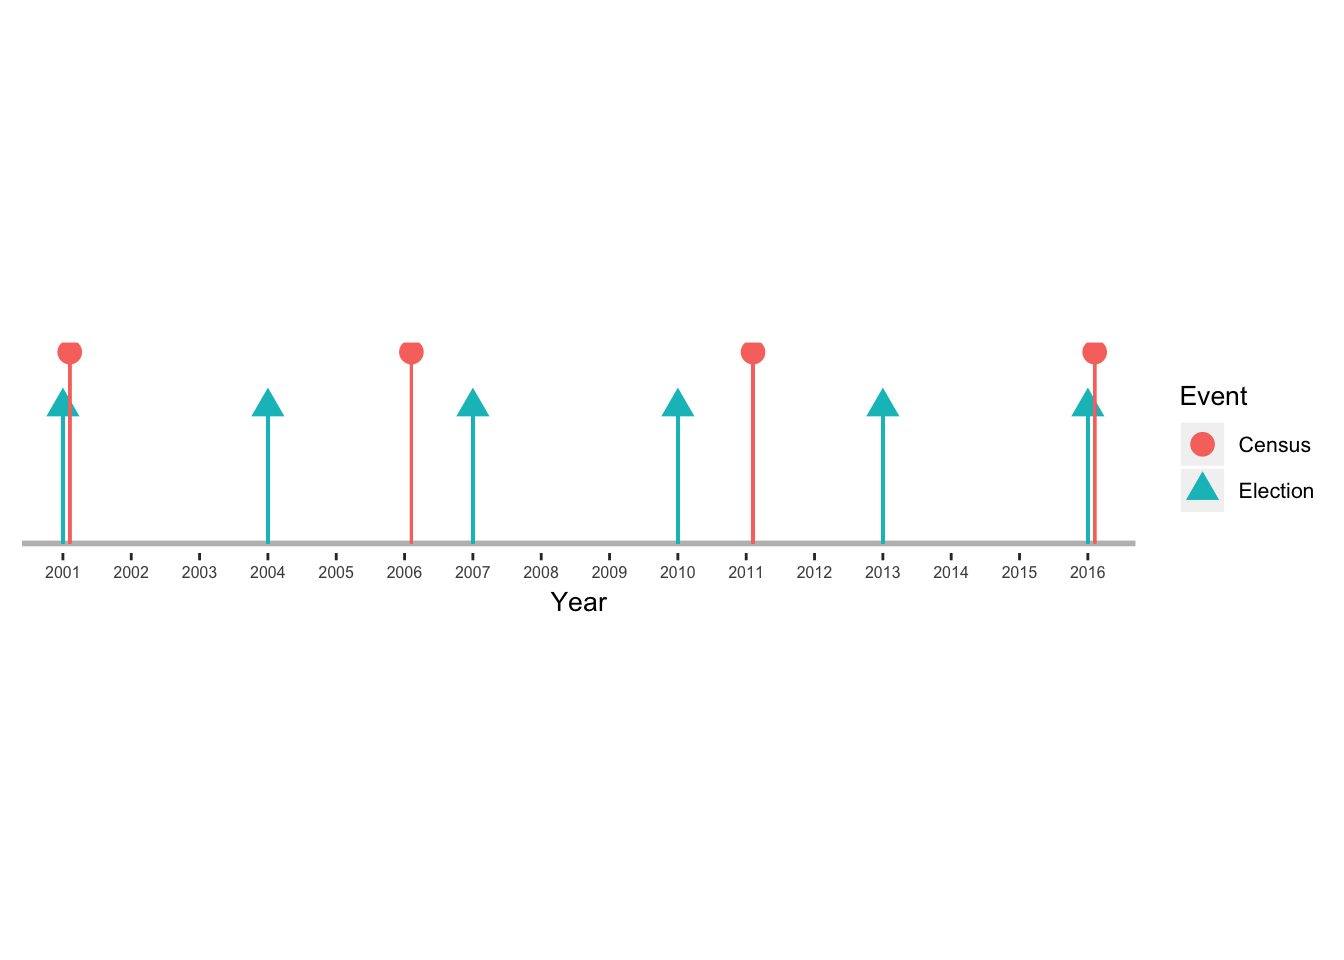
\includegraphics[width=0.9\linewidth]{draft-paper_files/figure-latex/timeline-1} 

}

\caption{Timeline of Australian elections and Censuses. They do not always occur in the same year.}\label{fig:timeline}
\end{figure}

\hypertarget{spatio-temporal-imputation}{%
\subsubsection{Spatio-temporal imputation}\label{spatio-temporal-imputation}}

For each election, neighbouring Census information has to be combined in some way so that it represents the boundaries in place at the time of the election. This is done by taking the electoral boundaries and imputing the corresponding socio-demographic characteristics for each of neighbouring Censuses, thereby addressing the spatial aspect. Next, to deal with the temporal component, characteristics at the time of the election are constructed using linear interpolation between the spatially imputed neighbouring Census variables.

To account for spatial differences, the piece-wise approximation method in \textcite{Goodchild1993} is adopted. Consider a map of source zones \(s = 1,...,S\), for which socio-demographic information is available, and a set of target zones \(t = 1,...,T\) for which information is to be imputed. This is described in the context of a single election, and a single neighbouring Census.

Let the map of electoral boundaries at the time of a Census define the source zones, and let the boundaries at the time of the election be the target zones. Denote the area of intersection between a source zone \(s\) and a target zone \(t\) as \(A_{s,t}\). Additionally, let the population of the source zone \(s\) be \(U_s\) and the population of intersection between source zone \(s\) and target zone \(t\) be \(P_{s,t}\). The estimated population of intersection is given by:

\[\hat{P}_{s,t} = \frac{U_s*A_{s,t}}{\sum_{t=1}^T A_{s,t}}, \mbox{ for all } s=1,...,S \mbox{ and } t=1,...,T.\]
Note that this estimator implicitly assumes that populations are uniformly distributed within each source zone.

In order to calculate socio-demographic information for each of the target zones, a weighted average is taken using the estimated intersection populations as weights. Denote a given Census variable for the target zone by \(C_t\), and the same Census variable for the source zone as \(D_s\). Then, estimate \(C_t\) using:

\[\hat{C}_t = \frac{\sum_{s=1}^{S}{D_s*\hat{P}_{s,t}}}{\sum_{s=1}^{S}{\hat{P}_{s,t}}}, \mbox{ for each } t=1,...,T.\]
This concludes the spatial imputation of the socio-demographic characteristics for one target zone (a single electoral boundary), at time of only one of the neighbouring Censuses. This process is repeated for all of the target zones, and then for the other neighbouring Census.

To account for temporal changes, linear interpolation is used between Census years to get the final estimate of a Census variable for the target zone in the election year. Let \(y_1\) be the year of the Census preceding an election, let \(y_2\) be the year of the election and \(y_3\) be the year of the Census that follows. Add this year subscript to the Census variable estimate \(\hat{C}_t\), resulting in \(\hat{C}_{t,y}\). Linear interpolating between these Census years results an imputed value for the election year, given by

\[\hat{C}_{t,y_2} = \frac{y_3-y_2}{y_3-y_1}*\hat{C}_{t,y_1} + \frac{y_2-y_1}{y_3-y_1}*\hat{C}_{t,y_3}.\]
Implicitly this assumes that population characteristics change in a linear manner over time.

\hypertarget{an-illustration-of-the-spatio-temporal-imputation}{%
\subsubsection{An illustration of the spatio-temporal imputation}\label{an-illustration-of-the-spatio-temporal-imputation}}

Census data is publicly available that different levels of aggregation, ranging from SA1 (over 50,000 zones) to electoral divisions (150 zones). For this study electoral divisions are used as source zones, and the imputation method is applied to produce socio-demographic variables for each of the 2004, 2007, 2010 and 2013 elections. As mentioned earlier, there is no need to impute socio-demographic variables for the 2001 and 2016 elections. To illustrate the method, consider the imputation of socio-demographic variables for the electorate of Hume in New South Wales (NSW) at the time of the 2013 federal election. The boundaries shown in Figure \ref{fig:hume13} define all target zones in NSW for 2013, with the target zone of interest (Hume) shaded purple.

\begin{figure}[h]

{\centering 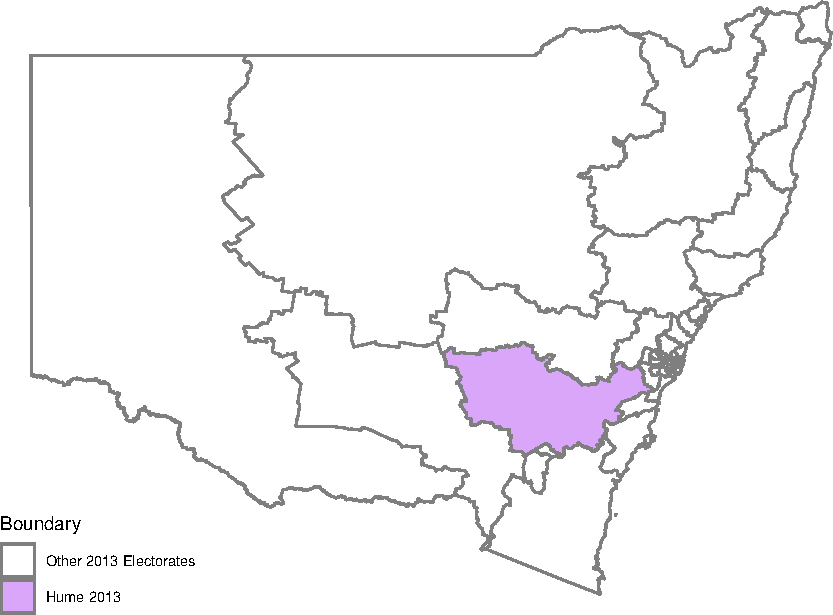
\includegraphics[height=0.3\textheight]{draft-paper_files/figure-latex/hume13-1} 

}

\caption{Some of the electoral boundaries in NSW for 2013, with the electoral boundary for Hume shown in purple.}\label{fig:hume13}
\end{figure}

The corresponding source zones from the 2016 Census are shown in Figure \ref{fig:hume16}. As can be seen, the Hume boundary from the 2013 election (shaded purple) does not perfectly match any of the source zones.

\begin{figure}[h]

{\centering 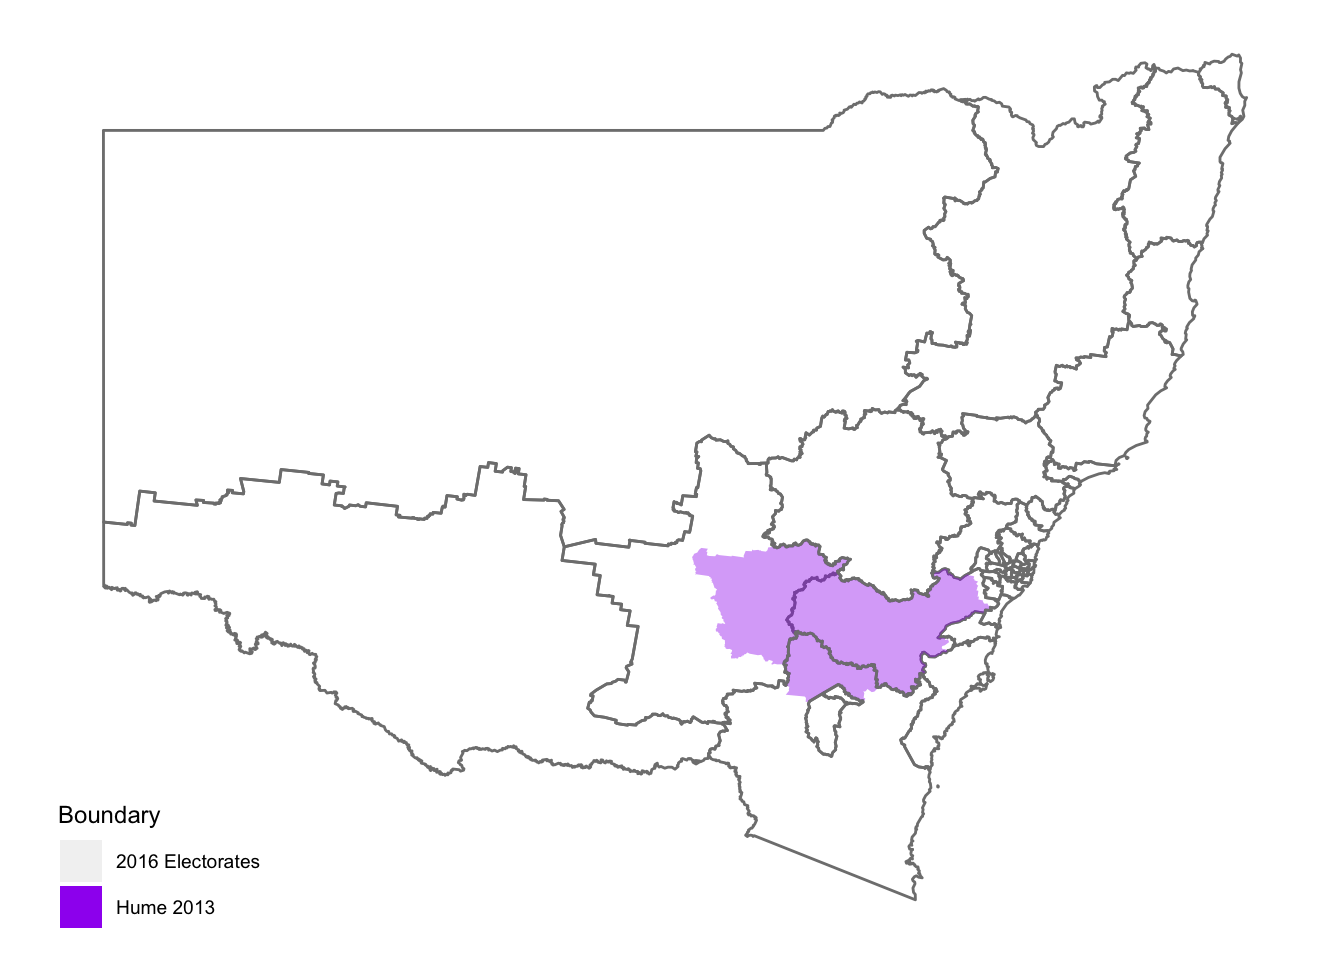
\includegraphics[height=0.3\textheight]{draft-paper_files/figure-latex/hume16-1} 

}

\caption{Census division boundaries in NSW for 2016, with the 2013 electoral boundary for Hume, shown in purple. The purple region is not contained within a single Census division.}\label{fig:hume16}
\end{figure}

There are many source zones from the 2016 Census that intersect with this purple region, including the divisions of Riverina, Eden-Monaro and Hume, along with smaller intersecting areas with Fenner, Calare, Gilmore and Whitlam. The proportion of each source zone that overlaps with the purple region is calculated, and used to obtain the intersecting populations \(\hat{P}_{s,t}\).

\footnotesize

\begin{longtable}[]{@{}llll@{}}
\toprule
\begin{minipage}[b]{0.21\columnwidth}\raggedright
Source Zone (2016)\strut
\end{minipage} & \begin{minipage}[b]{0.10\columnwidth}\raggedright
Proportion\strut
\end{minipage} & \begin{minipage}[b]{0.11\columnwidth}\raggedright
Source Zone Population\strut
\end{minipage} & \begin{minipage}[b]{0.46\columnwidth}\raggedright
Population Allocated to Purple Region: \(\hat{P}_{s,t}\)\strut
\end{minipage}\tabularnewline
\midrule
\endhead
\begin{minipage}[t]{0.21\columnwidth}\raggedright
HUME\strut
\end{minipage} & \begin{minipage}[t]{0.10\columnwidth}\raggedright
0.9654\strut
\end{minipage} & \begin{minipage}[t]{0.11\columnwidth}\raggedright
150643\strut
\end{minipage} & \begin{minipage}[t]{0.46\columnwidth}\raggedright
145427\strut
\end{minipage}\tabularnewline
\begin{minipage}[t]{0.21\columnwidth}\raggedright
RIVERINA\strut
\end{minipage} & \begin{minipage}[t]{0.10\columnwidth}\raggedright
0.2511\strut
\end{minipage} & \begin{minipage}[t]{0.11\columnwidth}\raggedright
155793\strut
\end{minipage} & \begin{minipage}[t]{0.46\columnwidth}\raggedright
39117\strut
\end{minipage}\tabularnewline
\begin{minipage}[t]{0.21\columnwidth}\raggedright
EDEN-MONARO\strut
\end{minipage} & \begin{minipage}[t]{0.10\columnwidth}\raggedright
0.1109\strut
\end{minipage} & \begin{minipage}[t]{0.11\columnwidth}\raggedright
147532\strut
\end{minipage} & \begin{minipage}[t]{0.46\columnwidth}\raggedright
16358\strut
\end{minipage}\tabularnewline
\begin{minipage}[t]{0.21\columnwidth}\raggedright
CANBERRA\strut
\end{minipage} & \begin{minipage}[t]{0.10\columnwidth}\raggedright
0.028\strut
\end{minipage} & \begin{minipage}[t]{0.11\columnwidth}\raggedright
196037\strut
\end{minipage} & \begin{minipage}[t]{0.46\columnwidth}\raggedright
548\strut
\end{minipage}\tabularnewline
\begin{minipage}[t]{0.21\columnwidth}\raggedright
FENNER\strut
\end{minipage} & \begin{minipage}[t]{0.10\columnwidth}\raggedright
0.0023\strut
\end{minipage} & \begin{minipage}[t]{0.11\columnwidth}\raggedright
202955\strut
\end{minipage} & \begin{minipage}[t]{0.46\columnwidth}\raggedright
474\strut
\end{minipage}\tabularnewline
\begin{minipage}[t]{0.21\columnwidth}\raggedright
WHITLAM\strut
\end{minipage} & \begin{minipage}[t]{0.10\columnwidth}\raggedright
0.0006\strut
\end{minipage} & \begin{minipage}[t]{0.11\columnwidth}\raggedright
152280\strut
\end{minipage} & \begin{minipage}[t]{0.46\columnwidth}\raggedright
92\strut
\end{minipage}\tabularnewline
\begin{minipage}[t]{0.21\columnwidth}\raggedright
GILMORE\strut
\end{minipage} & \begin{minipage}[t]{0.10\columnwidth}\raggedright
0.0006\strut
\end{minipage} & \begin{minipage}[t]{0.11\columnwidth}\raggedright
150436\strut
\end{minipage} & \begin{minipage}[t]{0.46\columnwidth}\raggedright
86\strut
\end{minipage}\tabularnewline
\begin{minipage}[t]{0.21\columnwidth}\raggedright
CALARE\strut
\end{minipage} & \begin{minipage}[t]{0.10\columnwidth}\raggedright
0.0001\strut
\end{minipage} & \begin{minipage}[t]{0.11\columnwidth}\raggedright
161298\strut
\end{minipage} & \begin{minipage}[t]{0.46\columnwidth}\raggedright
21\strut
\end{minipage}\tabularnewline
\bottomrule
\end{longtable}

\normalsize

Now consider the socio-demographic variable \(AusCitizen\) - the proportion of people in the region who are Australian citizens.

\footnotesize

\begin{longtable}[]{@{}lll@{}}
\toprule
\begin{minipage}[b]{0.26\columnwidth}\raggedright
Source Zone (2016)\strut
\end{minipage} & \begin{minipage}[b]{0.19\columnwidth}\raggedright
AusCitizen (\%): \(D_s\)\strut
\end{minipage} & \begin{minipage}[b]{0.47\columnwidth}\raggedright
Estimated Population Allocated to Purple Region: \(\hat{P}_{s,t}\)\strut
\end{minipage}\tabularnewline
\midrule
\endhead
\begin{minipage}[t]{0.26\columnwidth}\raggedright
HUME\strut
\end{minipage} & \begin{minipage}[t]{0.19\columnwidth}\raggedright
90.02\strut
\end{minipage} & \begin{minipage}[t]{0.47\columnwidth}\raggedright
145427\strut
\end{minipage}\tabularnewline
\begin{minipage}[t]{0.26\columnwidth}\raggedright
RIVERINA\strut
\end{minipage} & \begin{minipage}[t]{0.19\columnwidth}\raggedright
89.11\strut
\end{minipage} & \begin{minipage}[t]{0.47\columnwidth}\raggedright
39117\strut
\end{minipage}\tabularnewline
\begin{minipage}[t]{0.26\columnwidth}\raggedright
EDEN-MONARO\strut
\end{minipage} & \begin{minipage}[t]{0.19\columnwidth}\raggedright
88.00\strut
\end{minipage} & \begin{minipage}[t]{0.47\columnwidth}\raggedright
16358\strut
\end{minipage}\tabularnewline
\begin{minipage}[t]{0.26\columnwidth}\raggedright
CANBERRA\strut
\end{minipage} & \begin{minipage}[t]{0.19\columnwidth}\raggedright
85.48\strut
\end{minipage} & \begin{minipage}[t]{0.47\columnwidth}\raggedright
548\strut
\end{minipage}\tabularnewline
\begin{minipage}[t]{0.26\columnwidth}\raggedright
FENNER\strut
\end{minipage} & \begin{minipage}[t]{0.19\columnwidth}\raggedright
83.64\strut
\end{minipage} & \begin{minipage}[t]{0.47\columnwidth}\raggedright
474\strut
\end{minipage}\tabularnewline
\begin{minipage}[t]{0.26\columnwidth}\raggedright
WHITLAM\strut
\end{minipage} & \begin{minipage}[t]{0.19\columnwidth}\raggedright
89.52\strut
\end{minipage} & \begin{minipage}[t]{0.47\columnwidth}\raggedright
92\strut
\end{minipage}\tabularnewline
\begin{minipage}[t]{0.26\columnwidth}\raggedright
GILMORE\strut
\end{minipage} & \begin{minipage}[t]{0.19\columnwidth}\raggedright
89.03\strut
\end{minipage} & \begin{minipage}[t]{0.47\columnwidth}\raggedright
86\strut
\end{minipage}\tabularnewline
\begin{minipage}[t]{0.26\columnwidth}\raggedright
CALARE\strut
\end{minipage} & \begin{minipage}[t]{0.19\columnwidth}\raggedright
87.56\strut
\end{minipage} & \begin{minipage}[t]{0.47\columnwidth}\raggedright
21\strut
\end{minipage}\tabularnewline
\bottomrule
\end{longtable}

\normalsize

A weighted average of \(AusCitizen\), with the allocated population from each source zone as weights, yields \(\hat{C}_{Hume,2016} = 89.65 \%\). Repeating this process using the 2011 Census yields \(\hat{C}_{Hume,2011} = 91.00 \%\)

Finally, linear interpolation between 2011 and 2016 yields the 2013 estimate:
\begin{eqnarray*}
\hat{C}_{Hume,2013} & = &\frac{3}{5} \cdot \hat{C}_{Hume,2011} + \frac{2}{5} \cdot \hat{C}_{Hume,2016} \\
& = & \frac{3}{5} \cdot 91.00 \% + \frac{2}{5} \cdot 89.65 \% \\
& = & 90.46 \%
\end{eqnarray*}

This is done for each of the 65 socio-demographic variables, and is repeated for each of the 149 remaining target zones corresponding with 2013 electorates.

\hypertarget{modelling}{%
\section{Modelling}\label{modelling}}

Electoral socio-demographic variables are now available for each of the six elections and are joined with their corresponding two-party preferred votes. Before choosing an appropriate model, two issues with the socio-demographic variables are addressed. Firstly, variable scales change over the years, making it important to standardize variables. Secondly, many variables represent similar information and where appropriate, should be combined in some way. Principal component analysis is used to identify variables covary, from which intuitive groupings are selected to be combined into a single variable. This also reduces the dimension of the data. After these steps, a model specification is chosen.

\hypertarget{standardizing-variables}{%
\subsection{Standardizing variables}\label{standardizing-variables}}

Many of the socio-demographic variables have changing scales over the years. For example, inflation-adjusted median rental prices increased across almost all electorates, with median rent of 200 dollars per week placing an electorate in the 90th percentile in 2001, but only the 30th percentile in 2016. In order for socio-demographic effects to be comparable across years, all explanatory variables are standardized to have mean zero and variance one within each election year. By standardizing, each variable is reported as a relative measure compared to all other electorates in the same year.

\hypertarget{creating-factors}{%
\subsection{Creating factors}\label{creating-factors}}

There are only \(N = 150\) observations (electorates) in each election and \(p = 65\) socio-demographic variables in each cross-section, with many variables represent similar information about an electorate. Any model that uses all variables would face serious problems with multi-collinearity and over-fitting, which would likely lead to erroneous conclusions regarding variable significance. To address this, groups of variables that represent similar information are combined into ``factors''\footnote{A preliminary step involved removing all age bands, because age is represented by median age, and to remove variables relating to particular denominations of Christianity.}.

A factor is created from a group of variables if there is an intuitive reason as to why they should represent similar information and if there is evidence to suggest that they covary. For example, a potential group would be variables relating to electoral incomes - median family, household and personal incomes. To determine which variables covary, principal component analysis is used on a combined dataset of socio-demographic variables from all six elections. It is appropriate to compute principal components in this way because when computed separately for each election, scree plots level off after four components and the loadings of the first four components are similar across the elections.

Only the first four principal components from the combined dataset are considered, as the scree plot corresponding to the combined dataset levels off after the fourth component. Variables that have a large loading in a particular component are deemed to covary, with a loading with magnitude greater than 0.15 being considered large. Six factors are created using this criteria. These are; \texttt{Incomes} - median personal, household and family incomes, \texttt{Unemployment} - unemployment and labor force participation rates, \texttt{ProportyOwned} - rates of housing ownership, mortgages, renting and government housing, \texttt{RentLoanPrice} - median rental and loan repayments, \texttt{FamHouseSize} - average household size, ratio of people to families and household makeup (single person, couple with kids and couple without kids) and \texttt{Education} - high school and university qualifications, jobs requiring higher levels of education as well as vocational course completions and jobs that do not require higher education levels (e.g.~laborer, tradesperson). For each of these groups, variables with positive loadings are added and those with negative loadings are subtracted to create a factor. After computing these sums, each factor is standardized to have mean zero and variance one, within each election.

There are \(p=30\) variables in the resultant predictor set, with all of these used in the regression for each election.

\hypertarget{regression-incorporating-spatially-dependent-errors}{%
\subsection{Regression incorporating spatially dependent errors}\label{regression-incorporating-spatially-dependent-errors}}

An identical model specification is used for each of the six elections, with each election modelled separately. This allows for the socio-demographic effects to be estimated separately for each election year, facilitating analysis of temporal changes in variable effects. This approach is preferable to using a single longitudinal model because it avoids any concerns of undue bias stemming from incorrectly imposed time-varying restrictions on any variable. Without such restrictions, a pooled cross-sectional model does not yield any distinct advantage over separate cross-sections. The panel approach is avoided because of how frequently electoral boundaries change, noting that electorates with same name across elections are not guaranteed to represent the same geographical region. Therefore any fixed or random effects models would be difficult to estimate without implementing consistent boundaries, which would require further imputation.

For each cross-section, let the response \(\boldsymbol y\) be the vector two-party preferred vote in favour of the Liberal party, with \(y_i = 70\) representing a 70\% preference for Liberal, 30\% for Labor, in electorate \(i\). Although \(y_i\) lies in the interval \((0,100)\), observed values are never close to 0 or 100 (minimum \(24.05 \%\) and maximum \(74.90 \%\)), so there is no need to formally impose the constraint of \(y_i \in [0,100]\). Furthermore, the responses are found to be spatially correlated in each election (Moran's I test, \(p \le 7\cdot10^{-15}\)). This not surprising as electorates are aggregate spatial units, and hence the spatial structure of the data must modelled appropriately.

The spatial error model \autocite{Anselin88} is chosen because captures spatial heterogeneity by incorporating a spatially structured random effect vector \autocite{LeSage2009}. In this context, the random effect can be thought of as capturing the unobserved political climate in each electorate, where this climate is correlated with the climate in neighbouring electorates, under the assumption that the climate is independent of electoral socio-demographics.

Spatial weights are calculated in accordance with the assumption that an electorate is equally correlated with any electorate that shares a part of its boundary. Let \(\rho\) be spatial autoregressive coefficient, \(\boldsymbol v\) be a spherical error term, \({\boldsymbol W}\) be a matrix of spatial weights (containing information about the neighbouring regions), \(\boldsymbol X\) be a matrix of socio-demographic covariates, \(\boldsymbol \beta\) be a vector of regression coefficients and \(\boldsymbol a\) be a spatially structured random effect vector.

\[{\boldsymbol y} = {\boldsymbol X} {\boldsymbol \beta} + {\boldsymbol a},\]
and

\[{\boldsymbol a} = \rho {\boldsymbol W} {\boldsymbol a} + {\boldsymbol v},\]
where

\[{\boldsymbol v} \sim N({\boldsymbol 0}, \sigma^2 {\boldsymbol I_n}),\].

and hence

\[{\boldsymbol y} = {\boldsymbol X} {\boldsymbol \beta} + ({\boldsymbol I}_n-\rho {\boldsymbol W})^{-1}{\boldsymbol v}.\]

Estimation of the above spatial error model is undertaken using feasible generalized least squares.

Table 3 details the estimated model coefficients and their estimated standard errors, for each of the six elections. An interpretation of these estimated values is provided in the next section.

\begin{table}[!htbp] \centering
  \caption{Estimated spatial error model parameters (standard errors) for each of the six election years.}
  \label{}
\scriptsize
\begin{tabular}{@{\extracolsep{1pt}}lcccccc}
\\[-1.8ex]\hline
 & 2001 & 2004 & 2007 & 2010 & 2013 & 2016 \\
\hline \\[-1.8ex]
 $\rho$ & 0.46$^{***}$ & 0.29$^{*}$ & 0.24 & 0.19 & 0.27$^{*}$ & 0.50$^{***}$ \\
  & (0.15) & (0.17) & (0.17) & (0.16) & (0.16) & (0.17) \\

 AusCitizen & $-$3.13 & $-$2.64 & $-$2.53 & $-$0.08 & $-$3.40 & $-$1.80 \\
  & (2.26) & (2.43) & (2.34) & (2.79) & (2.76) & (2.71) \\

 BornAsia & 2.22 & $-$0.95 & $-$1.60 & $-$6.83$^{**}$ & $-$3.03 & $-$0.55 \\
  & (2.18) & (2.44) & (2.19) & (2.73) & (2.71) & (2.17) \\

 BornMidEast & $-$1.15 & $-$1.59 & $-$2.01$^{*}$ & $-$2.03 & $-$0.92 & $-$1.44 \\
  & (1.07) & (1.20) & (1.11) & (1.27) & (1.24) & (1.13) \\

 BornSEEuro & $-$3.21$^{**}$ & $-$4.24$^{***}$ & $-$3.61$^{***}$ & $-$4.14$^{***}$ & $-$3.69$^{***}$ & $-$2.72$^{***}$ \\
  & (1.42) & (1.46) & (1.02) & (1.19) & (1.07) & (0.97) \\

 BornUK & 0.25 & $-$0.07 & 0.34 & 0.56 & $-$0.09 & $-$1.32 \\
  & (1.00) & (0.98) & (0.90) & (1.07) & (1.04) & (1.04) \\

 BornElsewhere & $-$5.04 & $-$4.91 & $-$4.13 & 2.35 & $-$5.23 & $-$4.14 \\
  & (3.30) & (3.68) & (3.38) & (4.23) & (4.15) & (3.97) \\

 Buddhism & $-$0.49 & $-$0.17 & $-$1.37 & $-$0.83 & $-$0.12 & $-$1.60 \\
  & (1.39) & (1.61) & (1.61) & (1.80) & (1.68) & (1.56) \\

 Christianity & $-$2.48 & $-$1.23 & 0.38 & 0.50 & 2.41 & 1.68 \\
  & (1.73) & (1.85) & (1.83) & (1.99) & (1.85) & (1.78) \\

 CurrentlyStudying & $-$2.19$^{**}$ & $-$0.13 & 2.06$^{*}$ & 2.12$^{*}$ & 1.15 & $-$0.16 \\
  & (0.99) & (1.13) & (1.17) & (1.25) & (1.26) & (1.18) \\

 DeFacto & $-$6.44$^{***}$ & $-$5.37$^{**}$ & $-$6.43$^{***}$ & $-$8.07$^{***}$ & $-$6.56$^{**}$ & $-$8.53$^{***}$ \\
  & (1.87) & (2.48) & (2.31) & (3.06) & (3.11) & (2.83) \\

 DiffAddress & 3.88$^{***}$ & 5.06$^{***}$ & 4.22$^{***}$ & 5.57$^{***}$ & 3.53$^{*}$ & 5.67$^{***}$ \\
  & (0.94) & (1.12) & (0.99) & (1.76) & (1.91) & (1.60) \\

 Distributive & 1.27 & 2.01$^{*}$ & 1.36 & 1.57 & 2.10$^{*}$ & 1.20 \\
  & (1.12) & (1.21) & (1.13) & (1.34) & (1.27) & (1.21) \\

 Education & 1.08 & 0.52 & $-$5.52$^{*}$ & $-$4.08 & $-$4.44 & $-$7.07$^{**}$ \\
  & (2.38) & (3.12) & (3.27) & (3.95) & (3.78) & (3.55) \\

 Extractive & 4.83$^{***}$ & 5.45$^{***}$ & 5.37$^{***}$ & 7.31$^{***}$ & 6.71$^{***}$ & 7.43$^{***}$ \\
  & (1.48) & (1.42) & (1.36) & (1.56) & (1.47) & (1.39) \\

 FamHouseSize & $-$0.16 & 0.87 & $-$2.40 & $-$2.53 & $-$3.26 & $-$2.91 \\
  & (2.19) & (2.72) & (2.69) & (3.25) & (3.28) & (2.90) \\

 Incomes & 4.36$^{**}$ & 5.03$^{*}$ & 9.45$^{***}$ & 7.09$^{**}$ & 7.97$^{***}$ & 12.20$^{***}$ \\
  & (1.77) & (2.66) & (2.75) & (3.25) & (2.92) & (2.75) \\

 Indigenous & 2.91$^{*}$ & 1.97 & 2.48 & 2.84 & 0.67 & $-$0.05 \\
  & (1.68) & (1.95) & (1.75) & (2.16) & (2.14) & (2.00) \\

 Islam & $-$0.92 & $-$0.97 & $-$0.54 & $-$2.50 & $-$0.82 & $-$0.95 \\
  & (1.22) & (1.36) & (1.27) & (1.52) & (1.42) & (1.34) \\

 Judaism & 1.88$^{*}$ & 1.78 & 2.66$^{***}$ & 1.97$^{*}$ & 2.74$^{**}$ & 1.65$^{*}$ \\
  & (1.05) & (1.13) & (1.01) & (1.15) & (1.10) & (1.00) \\

 ManagerAdmin & 2.06$^{***}$ & 3.32$^{***}$ & 6.00$^{***}$ & 5.47$^{***}$ & 5.04$^{***}$ & 5.78$^{***}$ \\
  & (0.71) & (0.93) & (0.90) & (1.08) & (1.03) & (1.06) \\

 Married & 0.44 & 0.11 & $-$1.22 & $-$0.22 & 0.91 & $-$2.34 \\
  & (2.31) & (2.96) & (2.83) & (3.15) & (3.03) & (2.81) \\

 MedianAge & 2.32$^{*}$ & 4.96$^{***}$ & 3.66$^{**}$ & 4.00$^{*}$ & 2.30 & 2.87 \\
  & (1.32) & (1.65) & (1.81) & (2.26) & (2.08) & (1.79) \\

 NoReligion & $-$1.57 & $-$0.92 & 0.56 & $-$0.30 & 1.02 & 1.31 \\
  & (1.59) & (1.71) & (1.73) & (1.92) & (1.94) & (2.04) \\

 OneParentHouse & $-$1.73 & $-$0.45 & $-$0.75 & $-$1.46 & $-$0.77 & $-$0.74 \\
  & (1.36) & (1.59) & (1.49) & (1.69) & (1.57) & (1.47) \\

 OtherLanguage & $-$0.44 & 5.92 & 9.98$^{**}$ & 11.24$^{**}$ & 9.00$^{*}$ & 9.84$^{**}$ \\
  & (3.22) & (4.16) & (3.91) & (4.76) & (4.66) & (4.44) \\

 PropertyOwned & $-$0.46 & $-$0.53 & 0.67 & $-$0.94 & $-$0.48 & 1.41 \\
  & (1.37) & (1.50) & (1.43) & (1.76) & (1.67) & (1.50) \\

 RentLoanPrice & $-$1.57 & $-$3.32$^{*}$ & $-$4.01$^{**}$ & $-$0.97 & $-$0.70 & $-$0.89 \\
  & (1.49) & (1.76) & (1.67) & (2.07) & (2.07) & (2.16) \\

 SocialServ & 2.51$^{*}$ & 1.65 & 2.47$^{*}$ & 2.53$^{*}$ & 2.35$^{*}$ & 4.45$^{***}$ \\
  & (1.33) & (1.41) & (1.29) & (1.47) & (1.32) & (1.19) \\

 Transformative & 3.24$^{**}$ & 4.73$^{***}$ & 4.84$^{***}$ & 4.46$^{**}$ & 3.56$^{**}$ & 4.58$^{***}$ \\
  & (1.55) & (1.78) & (1.74) & (1.98) & (1.78) & (1.53) \\

 Unemployment & $-$2.45$^{*}$ & $-$3.07$^{*}$ & 0.29 & 0.08 & 1.67 & 2.79$^{**}$ \\
  & (1.40) & (1.63) & (1.51) & (1.76) & (1.51) & (1.37) \\

 Constant & 50.81$^{***}$ & 52.60$^{***}$ & 47.31$^{***}$ & 49.93$^{***}$ & 53.51$^{***}$ & 50.49$^{***}$ \\
  & (0.71) & (0.58) & (0.52) & (0.57) & (0.58) & (0.80) \\

\hline \\[-1.8ex]
Observations & 150 & 150 & 150 & 150 & 150 & 150 \\
Residual Standard Error (GLS) & 4.69 & 5.04 & 4.79 & 5.63 & 5.18 & 4.88 \\
\hline
\hline \\[-1.8ex]
\textit{Note:}  & \multicolumn{6}{l}{$^{*}$p$<$0.1; $^{**}$p$<$0.05; $^{***}$p$<$0.01} \\
\end{tabular}
\end{table}

\newpage

\hypertarget{results}{%
\section{Results}\label{results}}

\hypertarget{spatial-autoregressive-parameter}{%
\subsection{Spatial autoregressive parameter}\label{spatial-autoregressive-parameter}}

The spatial autoregressive coefficient \(\rho\) is positive and significant in only the 2001 and 2016 elections (Figure \ref{fig:rhovis}), meaning that, on average, in these elections, the political climate of an electorate appears to be affected by the attitudes of it's neighbours. Conversely, in the other four elections, the spatial effect weakens to become insignificant. In these years, it appears that the spatial component does not explain anything over and above the electoral socio-demographics, meaning electorates effectively voted independently.

\begin{figure}[h]

{\centering 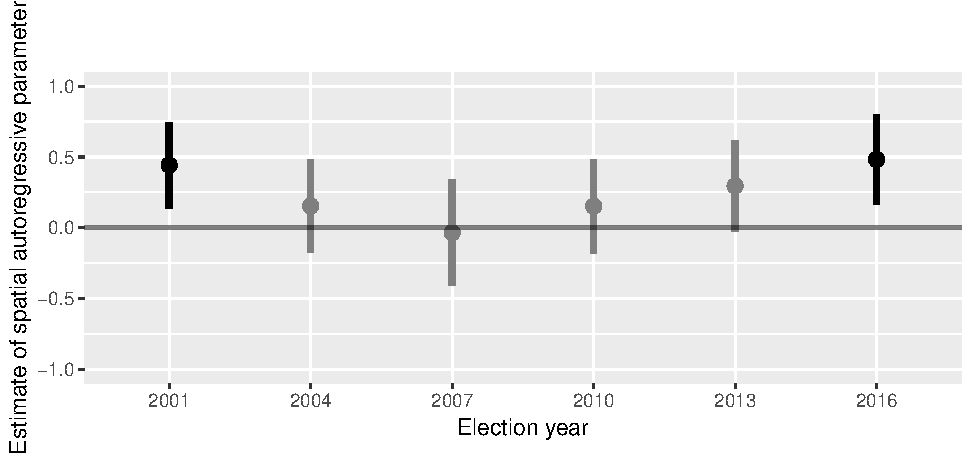
\includegraphics[height=0.15\textheight,]{draft-paper_files/figure-latex/rhovis-1} 

}

\caption{Estimates of the spatial autoregressive parameter for each of the six elections, reported with their individual 95\% confidence intervals. Only in 2001 and 2016 is there a significant spatial component.}\label{fig:rhovis}
\end{figure}

\hypertarget{country-wide-trend}{%
\subsection{Country-wide trend}\label{country-wide-trend}}

Since all socio-demographics have been standardized to have a mean of zero and a variance of one, the intercept in each model can be interpreted as the estimated two-party preferred vote for an electorate with mean characteristics\footnote{Mean of all variables aside from Judaism, Indigenous, Islam and Buddhism, where it assumes the mean of the log value.}. The baseline of party preference has varied over the elections, with the biggest swing occurring in the 2007 election where the mean electorate shifted more than five percentage points in favour of the Labor party.

\begin{figure}[h]

{\centering 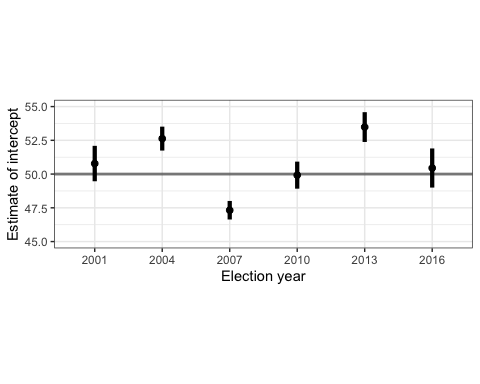
\includegraphics[height=0.15\textheight,]{draft-paper_files/figure-latex/plotintercept-1} 

}

\caption{Estimated intercept for each election, which represents the two-party preferred vote for an electorate with mean characteristics.}\label{fig:plotintercept}
\end{figure}

\hypertarget{influential-socio-demographics}{%
\subsection{Influential socio-demographics}\label{influential-socio-demographics}}

To investigate the socio-demographics that have a strong effect on the two-party preferred vote, partial residual plots are used and shown in Figures \ref{fig:partresplot1} and \ref{fig:partresplot2}. The partial residuals are the residuals from the fitted model with the estimated effect an individual variable added. These show the direction, size and significance of an estimated effect - the slope of the prediction line matches the estimated coefficient, and the shaded region represents a 95\% confidence band. If a horizontal line can be drawn through the confidence band, then the effect is insignificant. The estimated intercept is also added to the partial residuals for interpretability. Plots for each election are faceted to compare the effects over time in Figure \ref{fig:partresplot1} and Figure \ref{fig:partresplot2}.

It is important here to note the ecological fallacy: insights are being drawn at the electorate level, and cannot be inferred for another disaggregate level (e.g.~individual voters).

\hypertarget{income-and-unemployment}{%
\subsubsection{Income and unemployment}\label{income-and-unemployment}}

Typically the Labor party campaigns on more progressive policies, which often include tax reform that adversely affects higher income earners, and more generous social assistance programs. Perhaps it is due to these policies, that higher income electorates appear more likely to support the Liberal party, as the \texttt{Incomes} factor has a positive effect on Liberal preference (see row 1 in Figure \ref{fig:partresplot1}). This effect is significant in every election aside from 2004, where it is only marginally insignificant (\(p = 0.0613\)). Unemployment however, is not as influential. In 2001 and 2004, electorates with higher unemployment align with Labor, but over time this shifts towards support for the Liberal party, culminating in a significantly positive effect in 2016.

\hypertarget{industry-and-type-of-work}{%
\subsubsection{Industry and type of work}\label{industry-and-type-of-work}}

Electorates with higher proportions of workers in mining, gas, water, agriculture, waste and electricity (grouped as \texttt{Extractive} industries) are consistently linked with higher support for the Liberal party, with the magnitude of this effect slightly increasing over the years (see row 3 in Figure \ref{fig:partresplot1}). This is unsurprising, as the Liberal party has close ties with these traditional energy industries, and typically present policies to reduce taxation on energy production. Furthermore, electorates with more workers in construction or manufacturing industries (\texttt{Transformative}) are also more likely to support the Liberal party (see row 4 in Figure \ref{fig:partresplot1}).

Similarly, workers in managerial, administrative, clerical and sales roles (\texttt{ManagerAdmin}) is also a significant predictor of two-party preference vote across all six elections, with a higher proportion of people working these jobs increasing Liberal support. The magnitude of this effect also seems to increase over the years.

\hypertarget{household-mobility}{%
\subsubsection{Household mobility}\label{household-mobility}}

In each of the six elections, electorates with a higher proportion of people that have recently (past five years) moved house are more likely to support the Liberal party, although this effect was marginally insignificant in 2013 (see row 6 in Figure \ref{fig:partresplot1}. Having controlled for characteristics of house ownership and rental prices (via the factors \texttt{PropertyOwned} and \texttt{RentLoan} respectively), this is effect is somewhat surprising.

\hypertarget{relationships}{%
\subsubsection{Relationships}\label{relationships}}

De facto relationships, but not marriages, are found to be an important (and significant) predictor of the two-party preferred vote in all six elections, with more de facto relationships associated with higher support for the Labor party. The proportion of individuals who are marriages however, are insignificant (not shown).

\hypertarget{age}{%
\subsubsection{Age}\label{age}}

Regions comprised of older people are often believed to be more conservative, and indeed it found that electorates with a higher median age are more likely to support the Liberal party - although this effect is only significant in 2007 and 2010 (see row 2 in Figure \ref{fig:partresplot2}).

\hypertarget{education}{%
\subsubsection{Education}\label{education}}

Since 2007, electorates with higher education levels are associated with supporting the Labor party, although this effect is only significant in 2016. Before 2007, education has an almost zero effect (see row 3 in Figure \ref{fig:partresplot1}).

\hypertarget{diversity}{%
\subsubsection{Diversity}\label{diversity}}

Larger migrant populations from Asia, the Middle East, South-Eastern Europe, the United Kingdom and elsewhere, are either associated with Labor support, or have no effect. Of these areas, only South-Eastern European populations appear significant in each election, with the proportion of Asian migrants also being significant in 2010. Speaking other languages (aside from English) however, appears to have a far stronger effect, as observed through the \texttt{OtherLanguage} variable. Electorates with more diverse speech are associated with higher support for the Liberal party from 2004 onwards, with this effect being significant in 2007, 2010 and 2016. Furthermore, of the variables relating to religion, only Judaism shows a consistent effect, with electorates with relatively large Jewish populations more likely to vote Liberal.

\hypertarget{a-note-on-similar-variables}{%
\subsubsection{A note on similar variables}\label{a-note-on-similar-variables}}

Many of the Census variables represent similar information, which is why factors were created and some variables were removed. However, there still remain some variables which are closely related. For example, an electorate's income level (via \texttt{Incomes}) is likely to be related to electoral unemployment and labor force participation (via \texttt{Unemployment}). In 2001, the coefficient estimate for \texttt{Unemployment} is negative but not significant, whilst the \texttt{Incomes} variables is significant. If the \texttt{Incomes} variable is removed from the model in 2001, \texttt{Unemployment} absorbs the negative effect, becoming significant (\(p = 0.0056\)).

\hypertarget{a-closer-look-at-the-residuals}{%
\subsection{A closer look at the residuals}\label{a-closer-look-at-the-residuals}}

\hypertarget{residuals-by-state}{%
\subsubsection{Residuals by state}\label{residuals-by-state}}

It is often hypothesized that states have systematic differences that cause their electorates to vote differently. Boxplots of residuals grouped by state reveal that only Tasmania, the Australian Capital Territory and the Northern Territory appear to have a state-specific effect not captured by the models. Tasmania and the Australian Capital Territory appear to have a bias towards Labor, whereas the Northern Territory tends towards voting Liberal. However, there are relatively few electorates in each of these states (five, two and two respectively), so this apparent result may be due to incumbent effects rather than an actual state-specific bias.

\begin{figure}[h]

{\centering 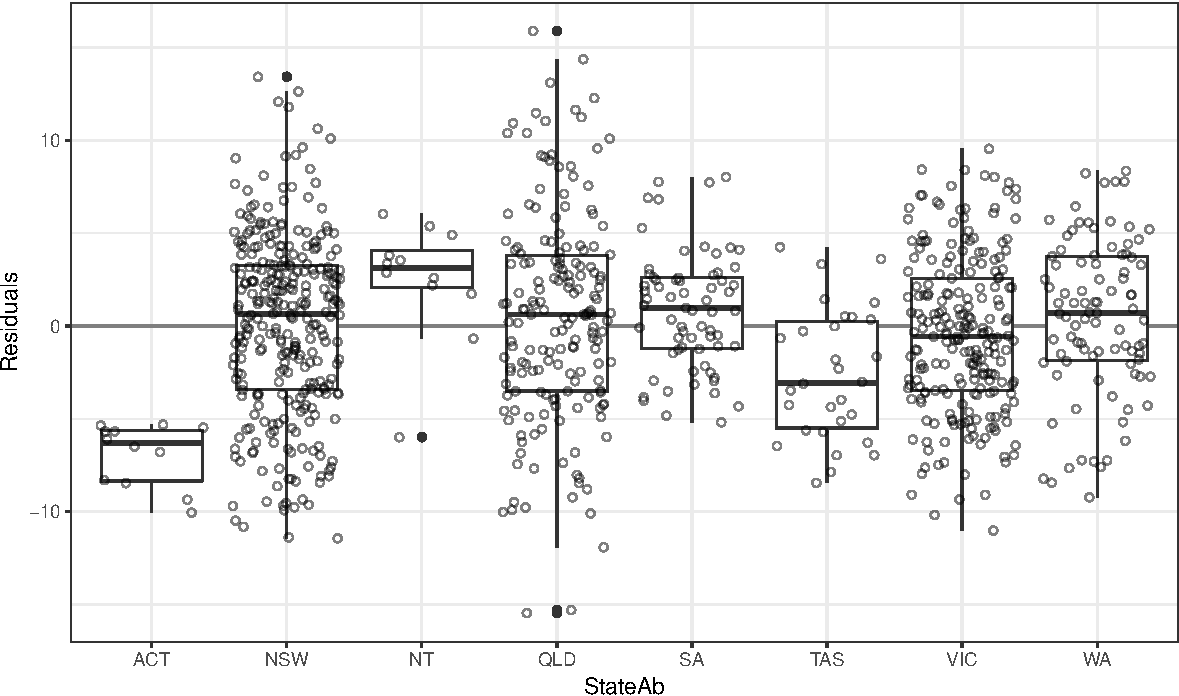
\includegraphics[width=0.7\linewidth,]{draft-paper_files/figure-latex/resstate-1} 

}

\caption{Boxplot of residuals by state with jittered points.}\label{fig:resstate}
\end{figure}

\hypertarget{outlier-electorates}{%
\subsubsection{Outlier electorates}\label{outlier-electorates}}

Based on the distribution of the Cook's distance values, a Cook's distance greater than \(0.1\) is considered to be influential and a potential outlier. The electorate of Sydney (NSW) has a large Cook's distance from 2001 to 2013, due to its diverse population (language, birthplace and religion), high number of defacto relationships, high income, high household mobility and small amount of workers in extractive and transformative jobs. It has remained a strong supporter of the Labor party and Liberal vote is severely overpredicted by the model, making it an outlier. Nearby in metropolitan NSW, the electorate of Wentworth is found to be an outlier in all but the 2007 election. Although historically Liberal, its two-party vote jumped by over 10 percentage points in 2010 without experiencing any notable changes in its socio-demographic makeup - implying that this may be the direct effect of its Liberal member, Malcolm Turnbull, becoming the leader of the Liberal party. Liberal support in Wentworth is underpredicted by the model in each year, and more so with Turnbull as Liberal leader.

Lingiari, an electorate taking up almost all of the Northern Territory, is an outlier in the 2001-2007 elections due to its large Indigenous population, young age profile and low rates of property ownership. Fowler (NSW) has a diverse population with a high proportion of migrants, many Buddhists and Muslims, and has strong Labor support, making it influential in 2001, 2004 and 2010. Other electorates with large Cook's distance are Barton (NSW) and Leichhardt (QLD) in 2016, and Canberra (ACT) in 2007.

\hypertarget{conclusion}{%
\section{Conclusion}\label{conclusion}}

This paper explores the effects of electoral socio-demographic characteristics on the two-party preferred vote in the 2001-2016 elections, using information from the corresponding Australian federal elections and Censuses. As a Census does not always occur in the same year as an election, Census data for the 2004-2013 elections are generated by employing a method of spatio-temporal imputation. This imputes electoral socio-demographics for the electoral boundaries in place at the time of the election - an approach that is distinctly different from previous work on modelling election outcomes, where Census and election data are typically joined without addressing their temporal differences. Before estimating a model, these socio-demographic variables are standardized (to adjust for changing variable scales) and many variables (representing similar information) are combined into factors, resulting in a reduced predictor set. A spatial error model is then fit for each election, accounting for the inherent spatial structure of the data.

Across the past six elections, most of the socio-demographics that drive the electoral two-party preferred vote are found to remain steady, whilst a few (typically weaker) effects vary over time. Industry and type of work are particularly influential, with energy-related and manufacturing/construction jobs, as well as administrative roles being strongly linked with the Liberal party in all elections. Incomes have a similarly consistent effect, with higher income areas supporting Liberal. Higher levels of unemployment shift from weak association with Labor to a significant Liberal effect over the years, and higher education levels are associated with Labor from 2007 (although only significant in 2016). It is also found that electorates with higher household mobility support Liberal, birthplace diversity favours Labor and more de facto relationships align with Labor preference - although marriages, family and household sizes have no material influence. Furthermore, the neighbourhood (spatial) effects are found to be positive in all elections, although only significant in 2001 and 2016, meaning that in the 2004-2013 elections, electorates effectively voted independently.

The findings in this paper complement the existing literature by modelling temporal trends, which as far as the authors are aware, has not been done previously for Australian elections using a regression framework. It is also the first study to model any Australian election since 2010 using Census information. Additionally, a key contribution of this research is the wrangling of the raw data and imputed data sets for the 2004, 2007, 2010 and 2013 elections, which have been contributed to the \texttt{eechidna} \texttt{R} package - providing a rich, accessible data resource for future Australian electoral analysis.

\hypertarget{acknowledgements}{%
\section{Acknowledgements}\label{acknowledgements}}

This paper was produced using \texttt{RMarkdown} \autocite{rmarkdown} and \texttt{knitr} \autocite{knitr}. All corresponding code for this paper can be found in the github repository (\url{https://github.com/jforbes14/journal-writing}), and the data used is available in the \texttt{eechidna} package \autocite{eechidna}. All raw data was obtained from the Australian Electoral Commission, the Australian Bureau of Statistics and the Australian Government.

\hypertarget{software}{%
\section{Software}\label{software}}

All election and Census datasets, along with electoral maps and more, are available in the \texttt{eechidna} \texttt{R} package, which can be downloaded from CRAN. \texttt{eechidna} (Exploring Election and Census Highly Informative Data Nationally for Australia) makes it easy to look at the data from the Australian Federal elections and Censuses that occurred between 2001 and 2016. This study contributed a large revision to the \texttt{eechidna} package, which included the addition of election and Census data for 2001-2010, voting outcomes for polling booths and imputed Census data for election years. For more details on using \texttt{eechidna}, please see the articles (vignettes) on the github page (\url{https://ropenscilabs.github.io/eechidna/}).

The authors would like to give a sincere thanks to Anthony Ebert, Heike Hofmann, Thomas Lumley, Ben Marwick, Carson Sievert, Mingzhu Sun, Dilini Talagala, Nicholas Tierney, Nathaniel Tomasetti, Earo Wang and Fang Zhou, all of whom have contributed to the \texttt{eechidna} package.

\begin{figure}[h]

{\centering 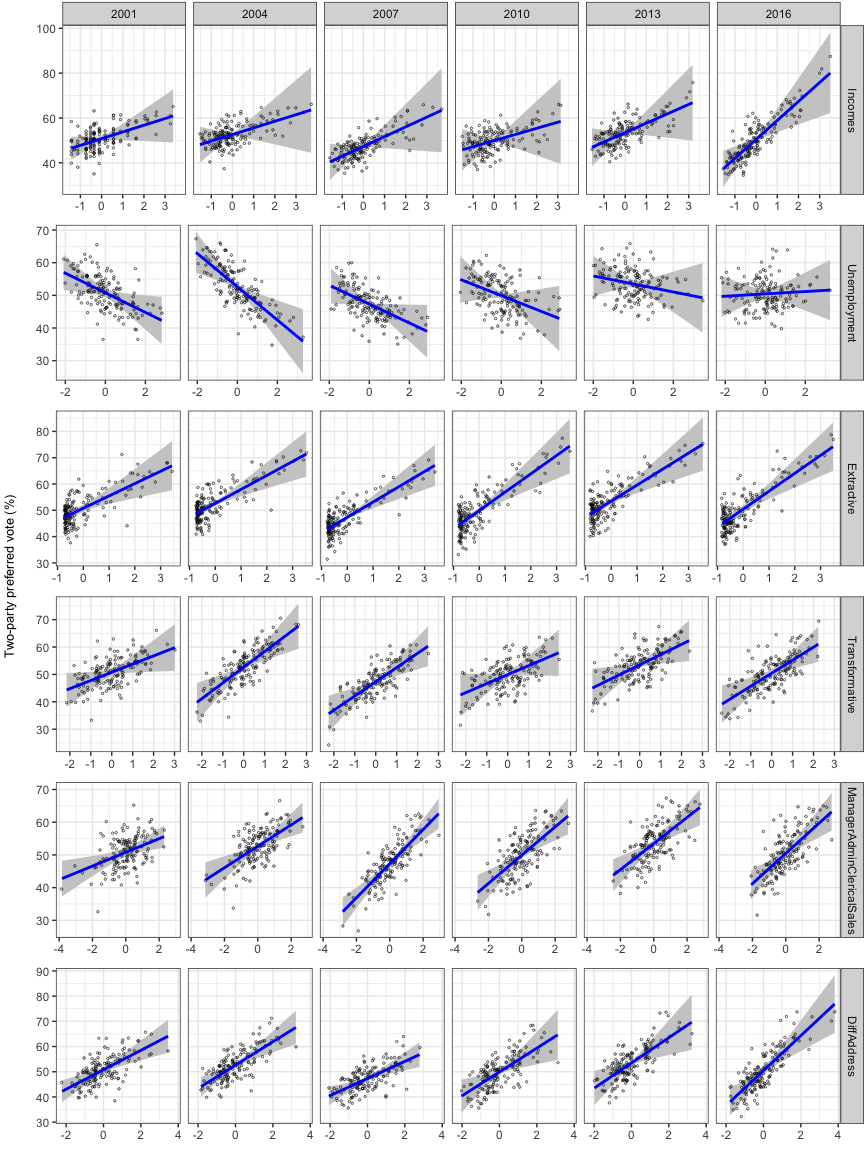
\includegraphics{draft-paper_files/figure-latex/partresplot1-1} 

}

\caption{Partial residual plots for: Incomes, Unemployment, Extractive, Transformative, ManagerAdmin and DiffAddress}\label{fig:partresplot1}
\end{figure}

\begin{figure}[h]

{\centering 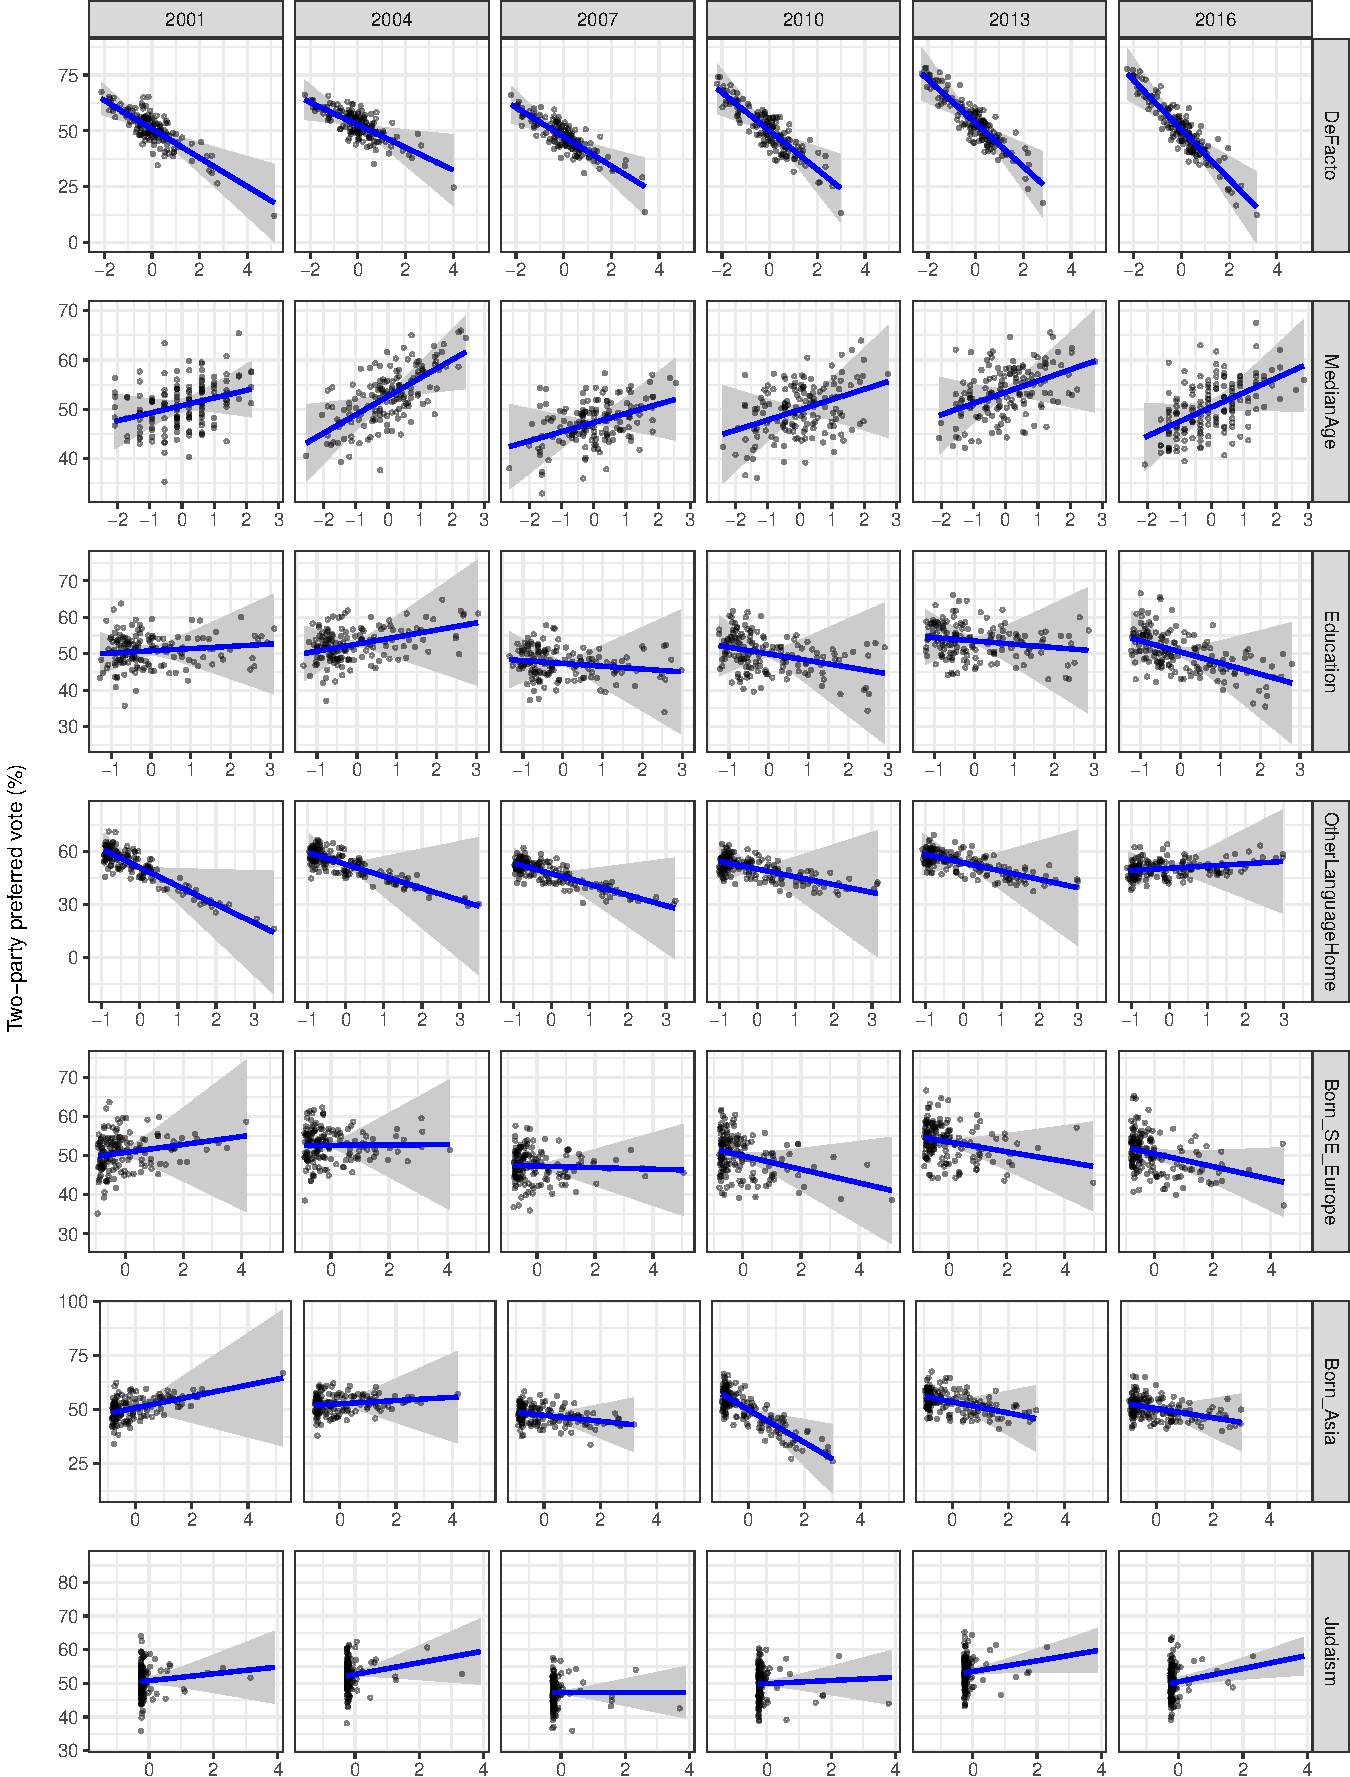
\includegraphics{draft-paper_files/figure-latex/partresplot2-1} 

}

\caption{Partial residual plots for: DeFacto, MedianAge, Education, OtherLanguage, BornSEEuro, BornAsia and Judaism.}\label{fig:partresplot2}
\end{figure}

\printbibliography

\end{document}
